\documentclass[preprint,amsmath,amssymb,aps, prb,showkeys]{revtex4-1}
\usepackage{graphicx}% Include figure files
\usepackage{bm}% bold math
\usepackage{color}
\usepackage{tabularx}
\usepackage{fullpage,subfigure,float,psfrag,textcomp,gensymb,tikz,siunitx}
\usepackage{booktabs,multirow, dcolumn}% Align table columns on decimal point
\usepackage{xspace}
\usepackage[bookmarks=true,pdftoolbar=true]{hyperref}
\hypersetup{%
  pdftitle = {MAX Phases: Supplementary text},
  pdfkeywords = {pdf, hyperref, bookmarks},
  pdfauthor = {Anjana Talapatra}}
 \usepackage[all]{hypcap} 

\def\etal{\mbox{\it et al.\ }} 
\newcommand{\eq}[1]{Eq.~\ref{#1}}
\newcommand{\fig}[1]{Fig.~\ref{#1}}
\newcommand{\tab}[1]{TABLE~\ref{#1}}

\begin{document}

\section{Supplementary material}
\label{sec:app}

\begin{figure}[h!]
\centering
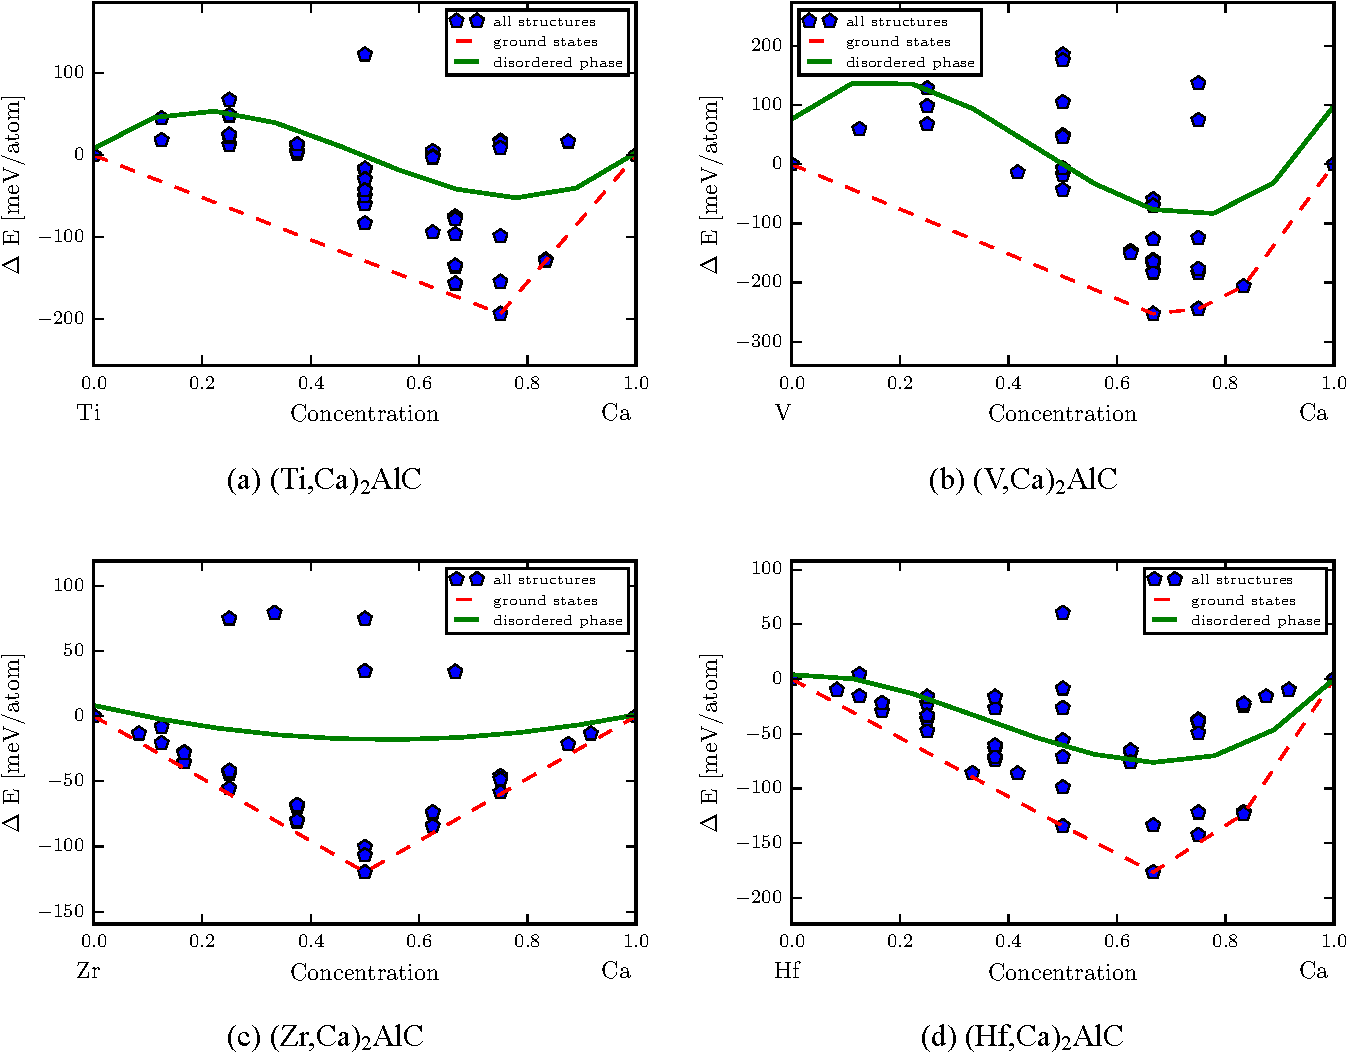
\includegraphics[scale=0.5]{figure_17.pdf}
\caption{Ground states at 0 K using cluster expansion for (M1,Ca)$_2$AlC, a) M1=Ti, b) M1=V, c) M1=Zr and d) M1=Hf }
\end{figure}

\begin{figure}
\centering
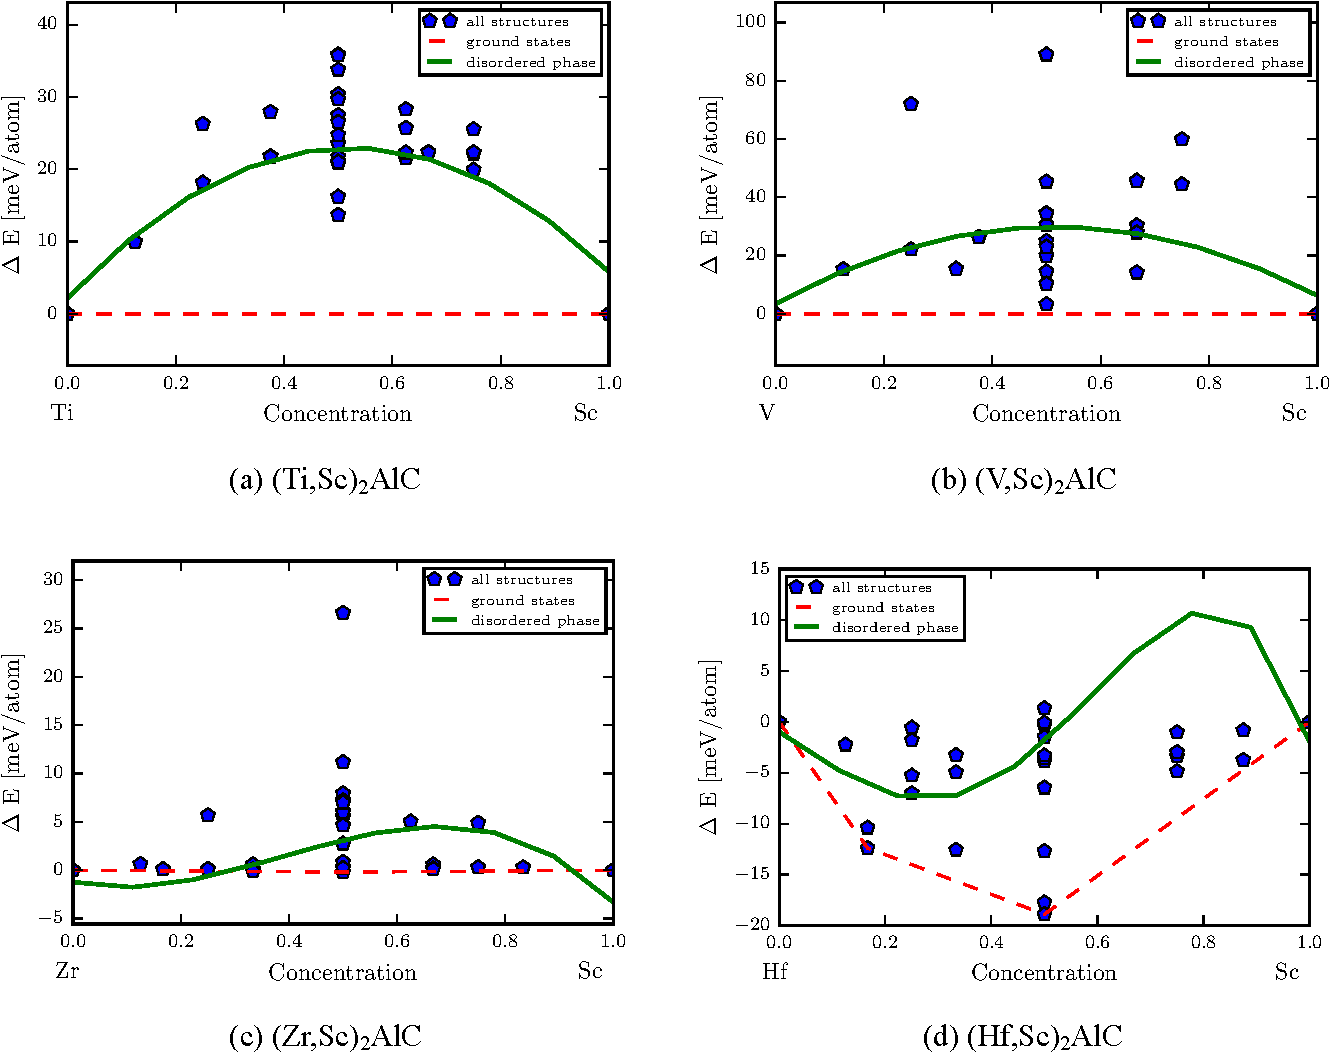
\includegraphics[scale=0.5]{figure_18.pdf} 
\caption{Ground states at 0 K using cluster expansion for (M1,Sc)$_2$AlC, a) M1=Ti, b) M1=V, c) M1=Zr and d) M1=Hf }
\end{figure}

\begin{figure}
\centering
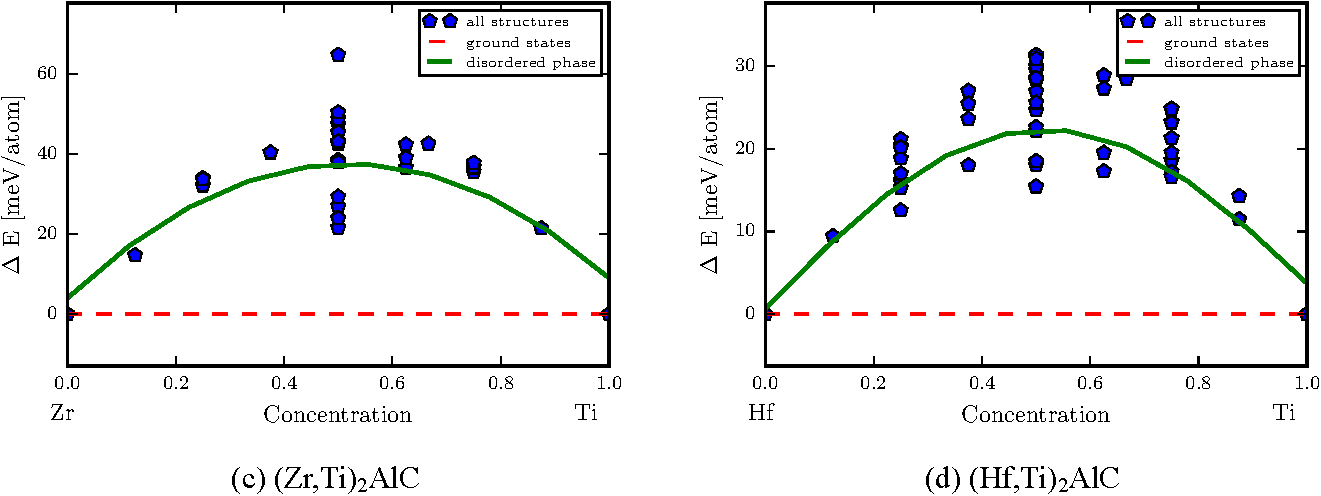
\includegraphics[scale=0.5]{figure_19.pdf}   
\caption{Ground states at 0 K using cluster expansion for (M1,Ti)$_2$AlC, a) M1=Zr, b) M1=Hf }
\end{figure}

\begin{figure}
\centering
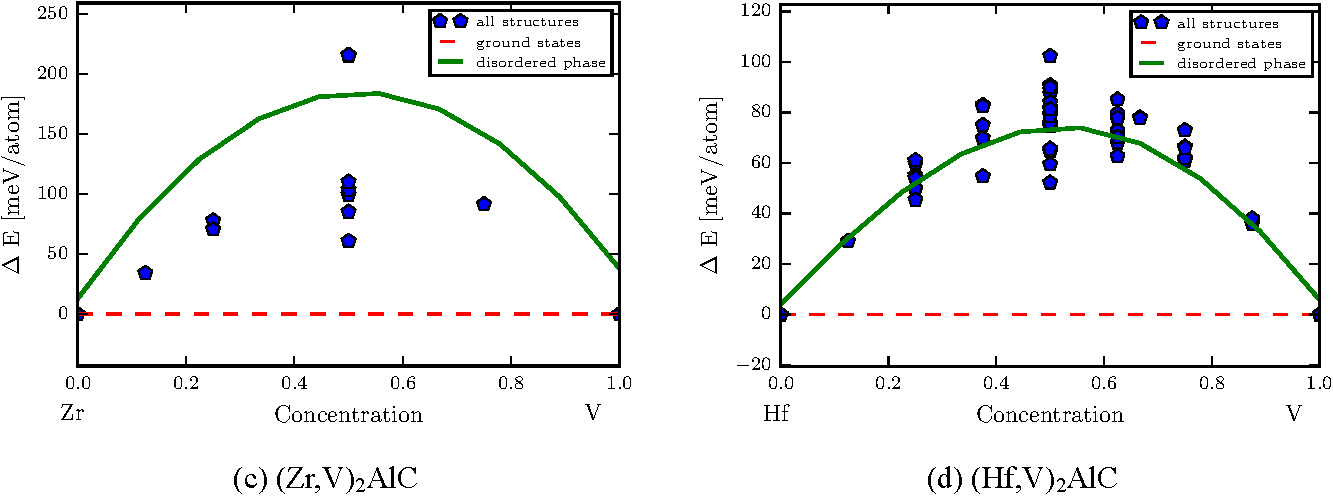
\includegraphics[scale=0.5]{figure_20.pdf}    
\caption{Ground states at 0 K using cluster expansion for (M1,V)$_2$AlC, a) M1=Zr, b) M1=Hf }
\end{figure}

\begin{figure}
\centering
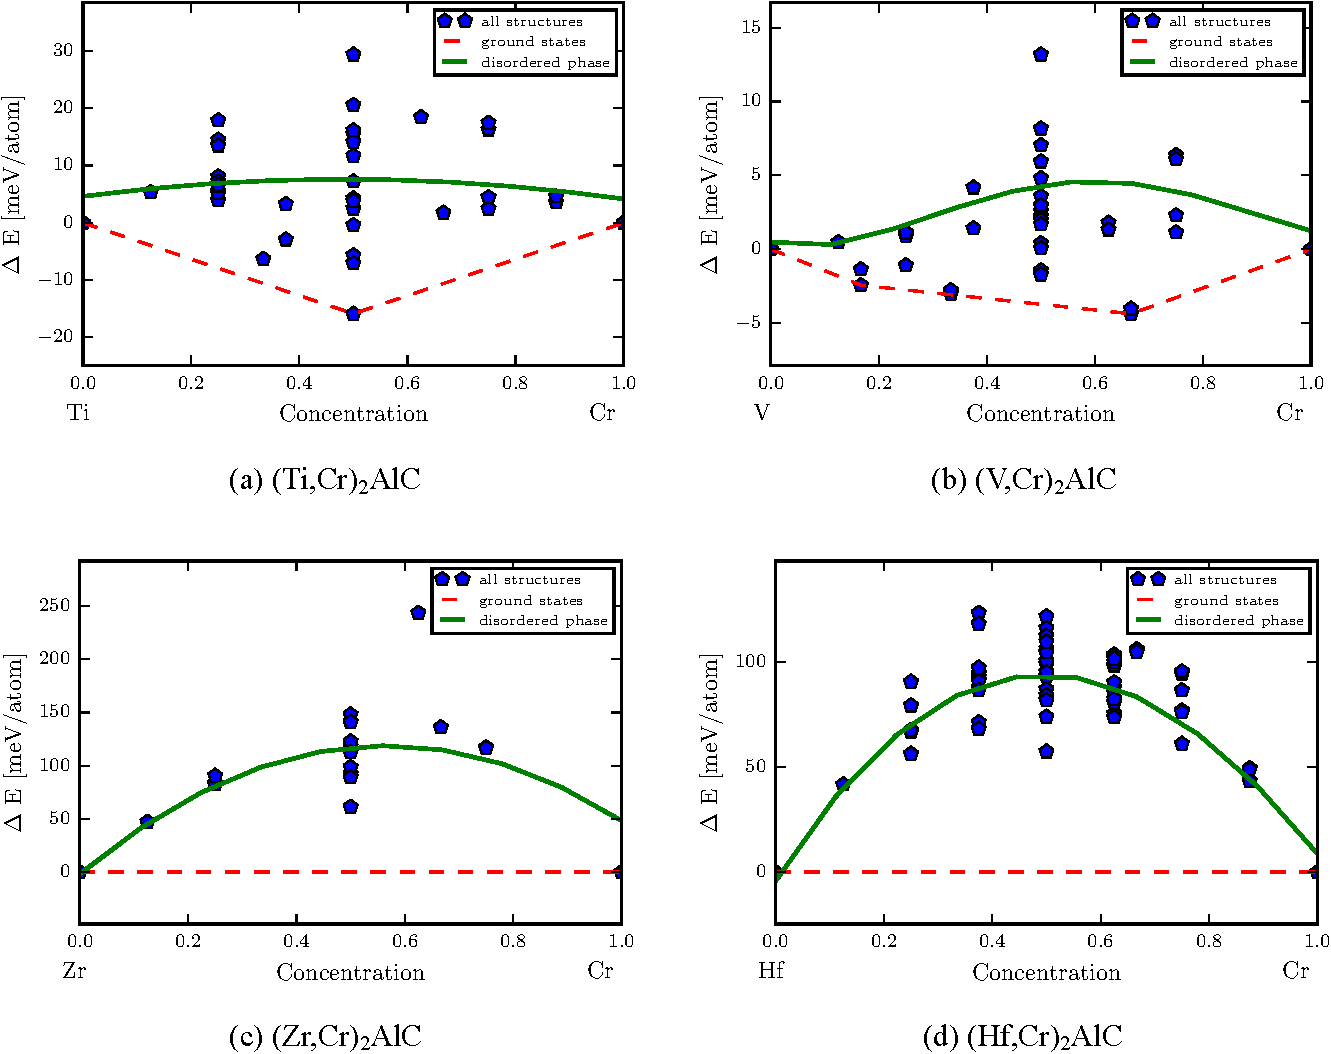
\includegraphics[scale=0.5]{figure_21.pdf}   
\caption{Ground states at 0 K using cluster expansion for (M1,Cr)$_2$AlC, a) M1=Ti, b) M1=V, c) M1=Zr and d) M1=Hf }
\end{figure}

\begin{figure}
\centering
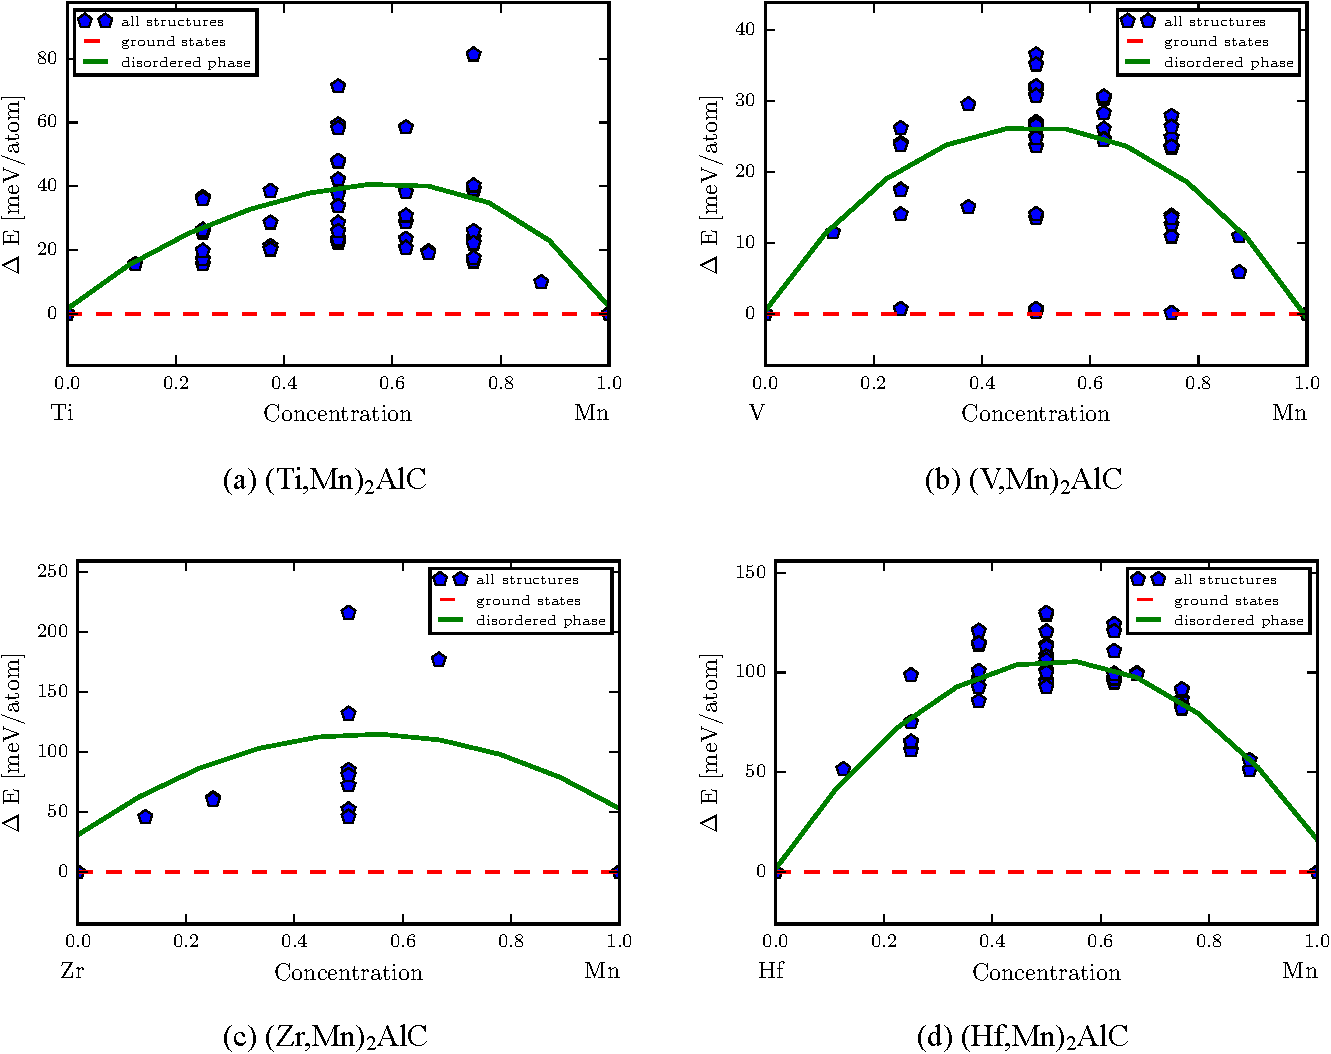
\includegraphics[scale=0.5]{figure_22.pdf}   
\caption{Ground states at 0 K using cluster expansion for (M1,Mn)$_2$AlC, a) M1=Ti, b) M1=V, c) M1=Zr and d) M1=Hf }
\end{figure}

\begin{figure}
\centering
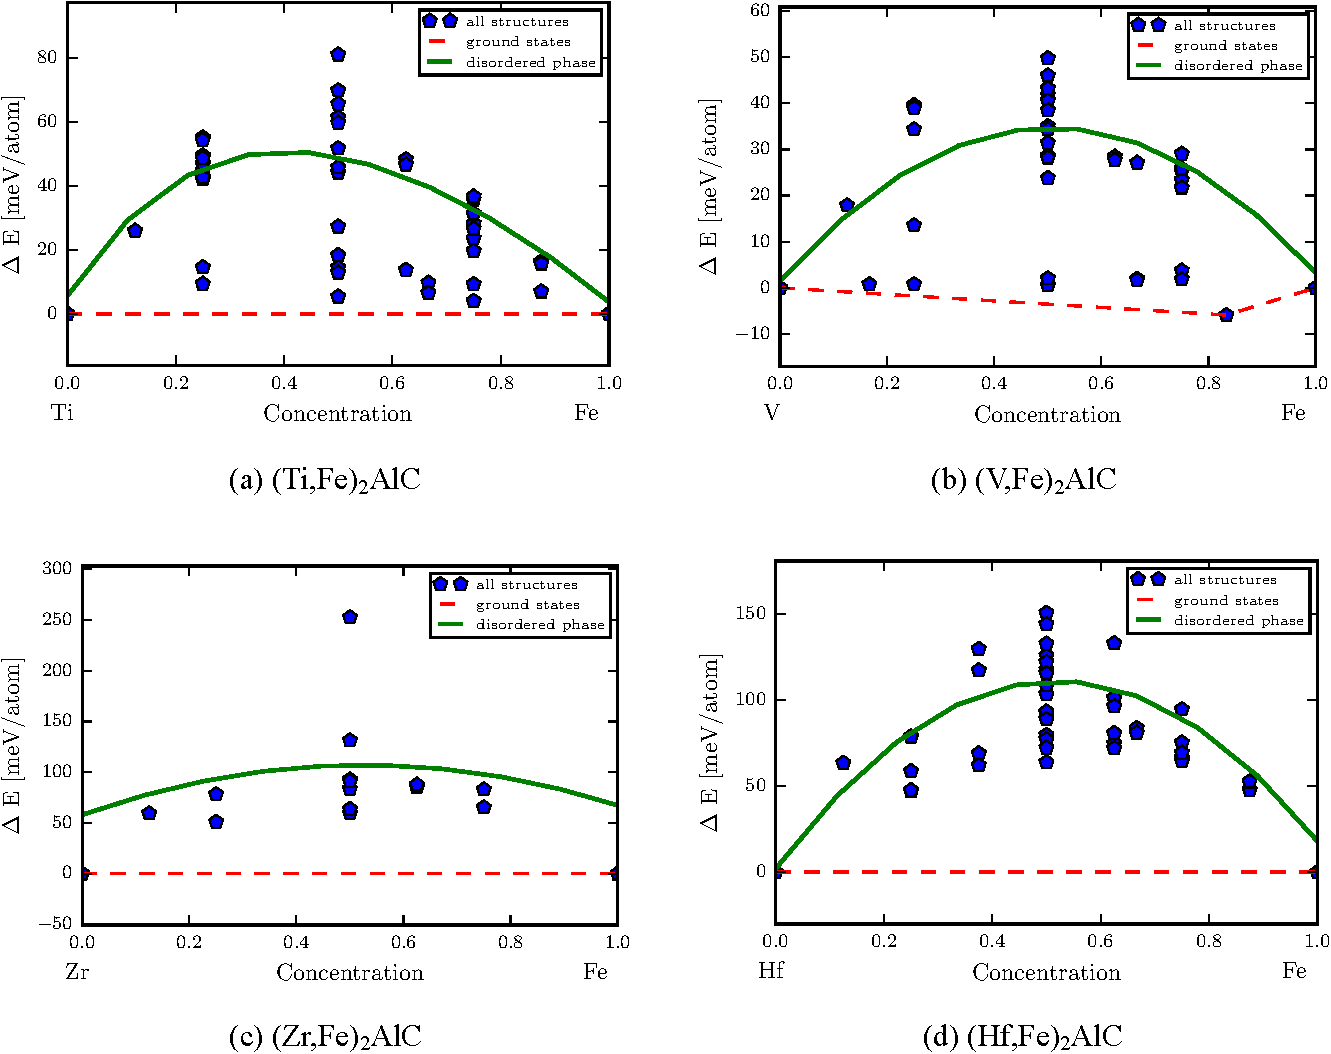
\includegraphics[scale=0.5]{figure_23.pdf}   
\caption{Ground states at 0 K using cluster expansion for (M1,Fe)$_2$AlC, a) M1=Ti, b) M1=V, c) M1=Zr and d) M1=Hf }
\end{figure}

\begin{figure}
\centering
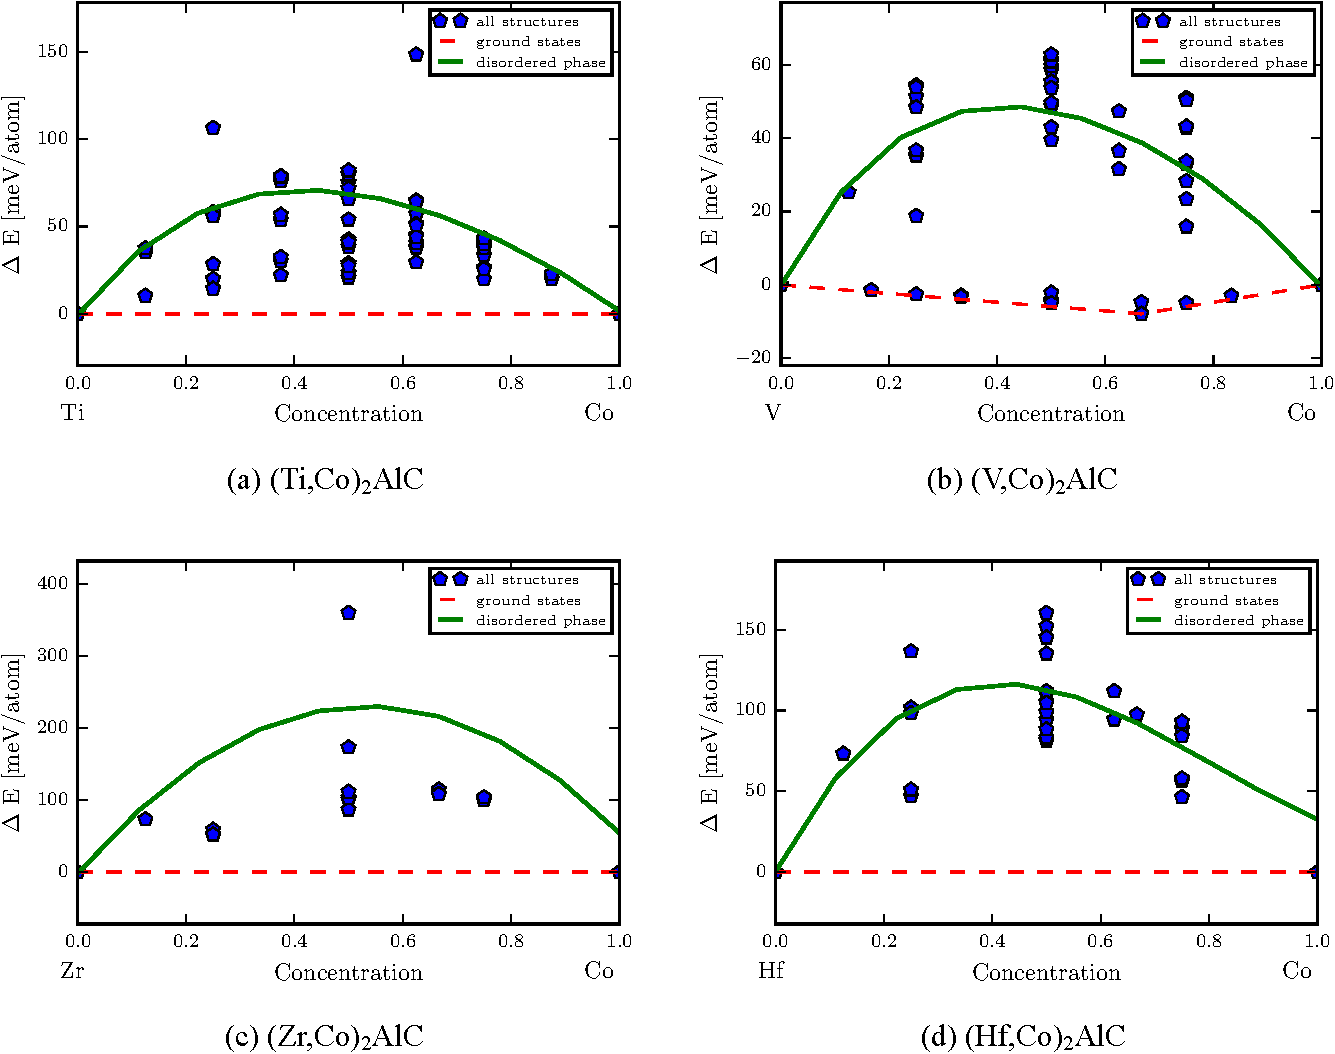
\includegraphics[scale=0.5]{figure_24.pdf}   
\caption{Ground states at 0 K using cluster expansion for (M1,Co)$_2$AlC, a) M1=Ti, b) M1=V, c) M1=Zr and d) M1=Hf }
\end{figure}

\begin{figure}
\centering
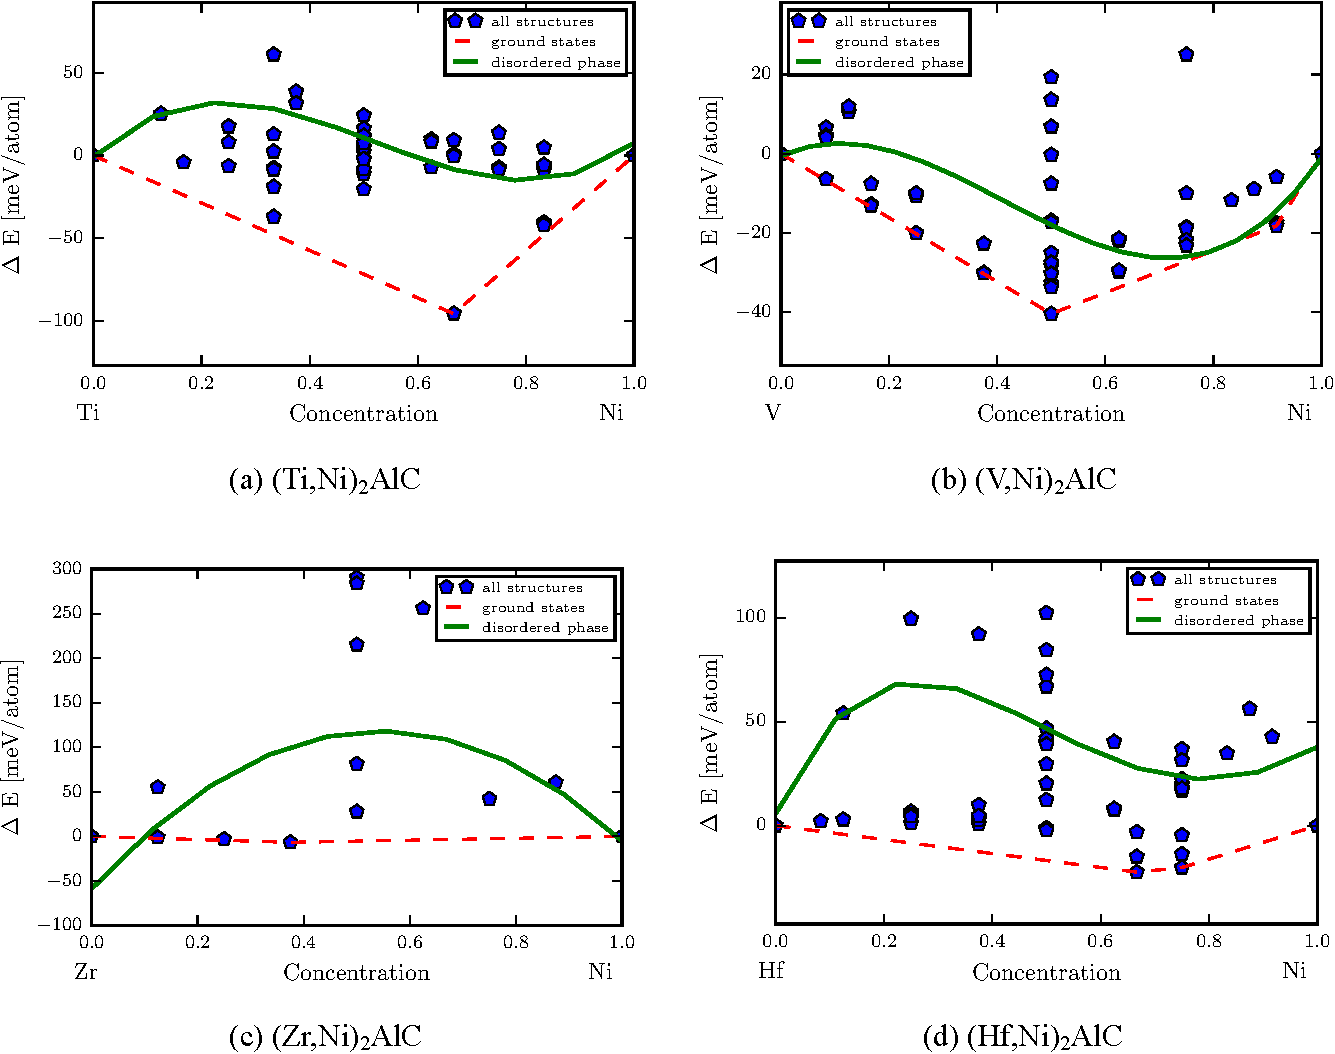
\includegraphics[scale=0.5]{figure_25.pdf}   
\caption{Ground states at 0 K using cluster expansion for (M1,Ni)$_2$AlC, a) M1=Ti, b) M1=V, c) M1=Zr and d) M1=Hf }
\end{figure}

\begin{figure}
\centering
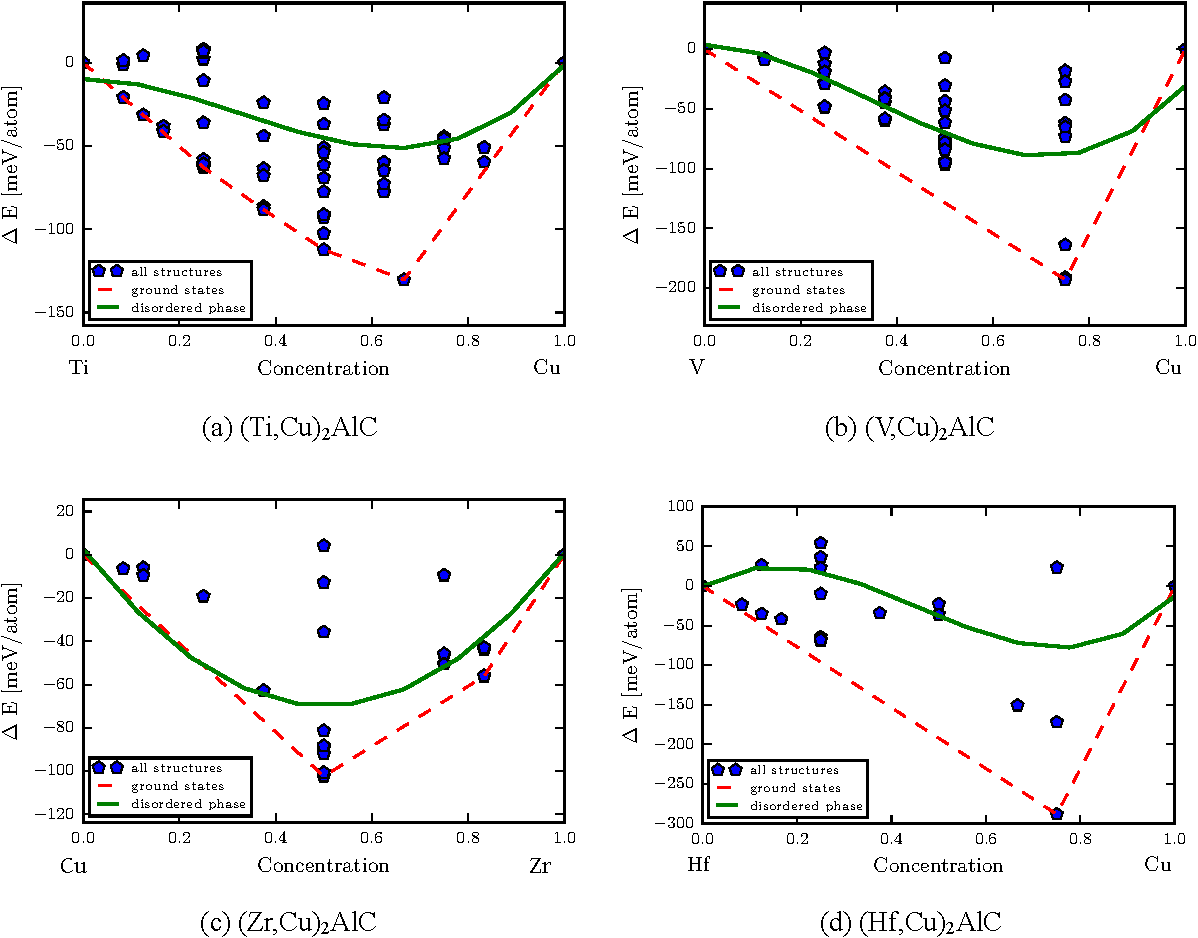
\includegraphics[scale=0.5]{figure_26.pdf}    
\caption{Ground states at 0 K using cluster expansion for (M1,Cu)$_2$AlC, a) M1=Ti, b) M1=V, c) M1=Zr and d) M1=Hf }
\end{figure}


\begin{figure}
\centering
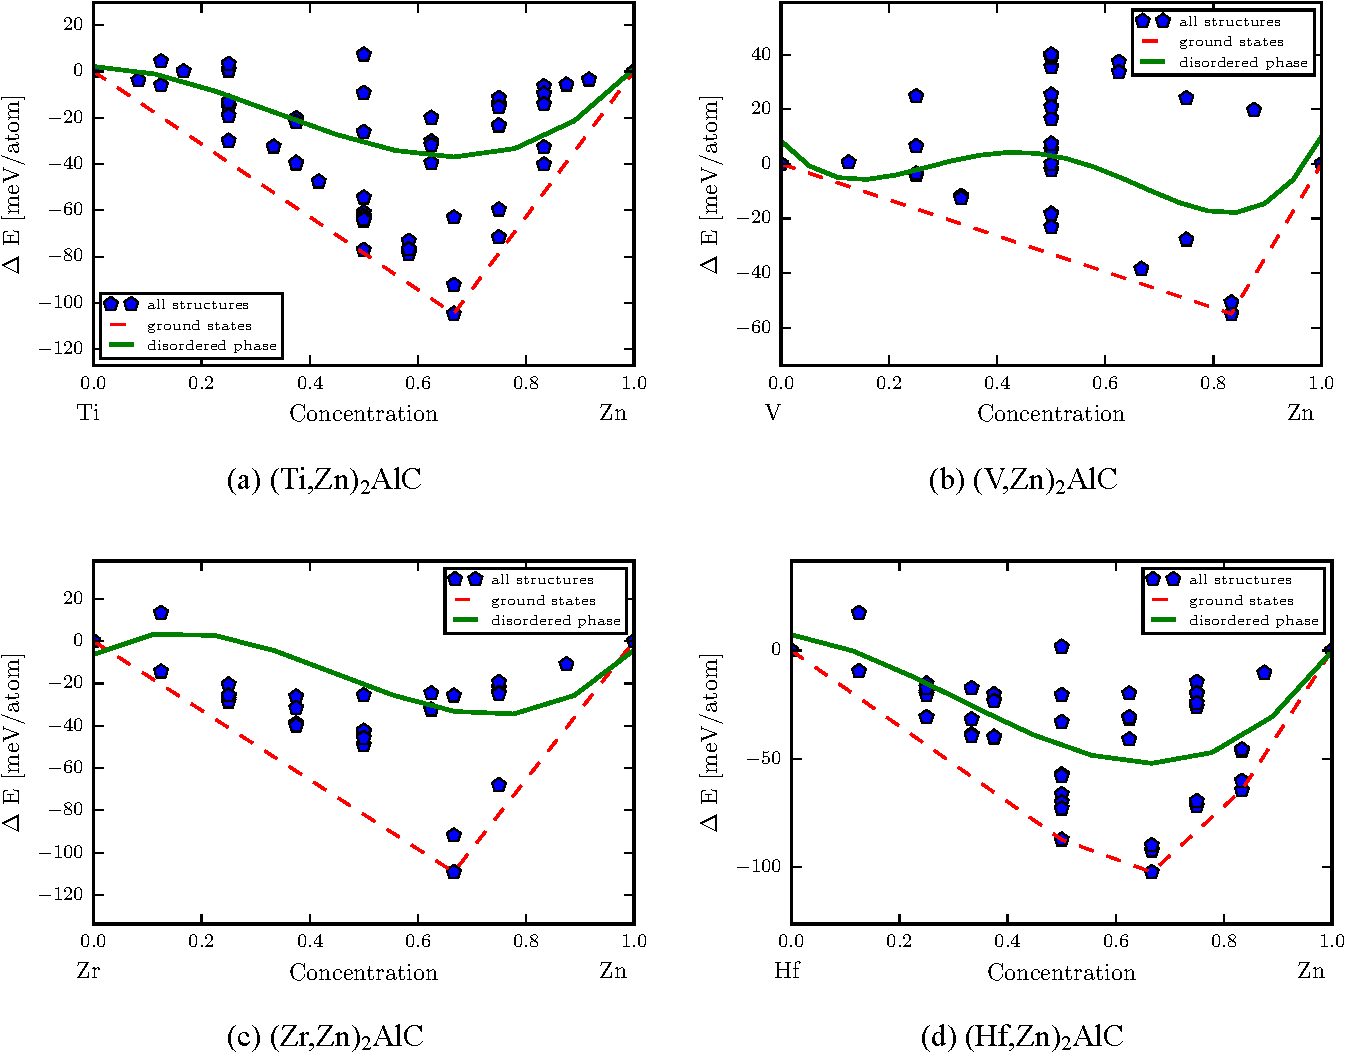
\includegraphics[scale=0.5]{figure_27.pdf}   
\caption{Ground states at 0 K using cluster expansion for (M1,Zn)$_2$AlC, a) M1=Ti, b) M1=V, c) M1=Zr and d) M1=Hf }
\end{figure}

\newpage

\begin{table}[htp!]
\centering
\setlength{\tabcolsep}{0.2cm}
\setlength\extrarowheight{6pt}
\begin{tabular}{clccccccc}
\hline
Sr. No & Composition                       & Space Group & a     & b     & c     & $\alpha$ & $\beta$ & $\gamma$ \\
\hline \hline
1      & (Ti$_{0.25}$Ca$_{0.75}$)$_2$AlC   & 31          & 3.79  & 7.19  & 13.18 & 90       & 90      & 90       \\
2      & (Ti${_0.5}$V${_0.5}$)$_2$AlC      & 62          & 2.97  & 5.17  & 13.48 & 90       & 90      & 90       \\
3	   & (Ti${_0.5}$Cr${_0.5}$)$_2$AlC     & 59          & 2.93  & 5.14  & 13.18 & 90       & 90      & 90       \\  
3      & (Ti$_{0.33}$Ni$_{0.67}$)$_2$AlC   & 15          & 5.22  & 12.12 & 12.12 & 78       & 78      & 60       \\
4      & (Ti$_{0.75}$Cu$_{0.25}$)$_2$AlC   & 156         & 3.10  & 3.10  & 13.08 & 90       & 90      & 120      \\
5      & (Ti$_{0.625}$Cu$_{0.375}$)$_2$AlC & 156         & 3.12  & 3.12  & 25.34 & 90       & 90      & 120      \\
6      & (Ti$_{0.50}$Cu$_{0.50}$)$_2$AlC   & 186         & 3.15  & 3.15 & 12.25  & 90       & 90      & 90       \\
7      & (Ti$_{0.33}$Cu$_{0.66}$)$_2$AlC   & 63          & 8.28  & 8.28 & 12.00  & 90       & 90      & 158      \\
8      & (Ti$_{0.34}$Zn$_{0.66}$)$_2$AlC   & 8           & 8.06  & 8.06  & 13.87 & 104      & 104     & 23       \\

\hline \hline
\end{tabular}
\caption{Space group, lattice paramters ( a, b, c in angstrom units) and lattice angles (in degrees)  of all identified ordered phases for M1=Ti}
\end{table}

\begin{table}[htp!]
\centering
\setlength{\tabcolsep}{0.2cm}
\setlength\extrarowheight{6pt}
\begin{tabular}{clccccccc}
\hline
Sr. No & Composition                      & Space Group & a     & b     & c     & $\alpha$ & $\beta$ & $\gamma$ \\
\hline \hline
1     & (V$_{0.17}$Ca$_{0.83}$)$_2$AlC    & 155         & 15.96 & 15.96 & 15.96 & 22       & 22      & 22       \\
2     & (V$_{0.25}$Ca$_{0.75}$)$_2$AlC    & 1           & 15.50 & 15.19 & 15.64 & 23       & 22      & 23       \\
3     & (V$_{0.34}$Ca$_{0.66}$)$_2$AlC    & 15          & 13.09 & 13.09 & 13.09 & 22       & 22      & 22       \\
4     & (V$_{0.34}$Cr$_{0.66}$)$_2$AlC    & 9           & 13.10 & 13.10 & 13.10 & 24       & 24      & 24       \\
5     & (V$_{0.83}$Cr$_{0.17}$)$_2$AlC    & 189         & 5.03  & 5.03  & 13.00 & 90       & 90      & 120      \\
6     & (V$_{0.83}$Fe$_{0.17}$)$_2$AlC    & 194         & 2.85  & 2.85  & 37.18 & 90       & 90      & 90       \\
7     & (V$_{0.34}$Co$_{0.66}$)$_2$AlC    & 194         & 2.88  & 2.88  & 36.86 & 90       & 90      & 120      \\
8     & (V$_{0.5}$Ni$_{0.5}$)$_2$AlC      & 62          & 2.97  & 4.77  & 12.92 & 90       & 90      & 90       \\
8     & (V$_{0.08}$Ni$_{0.92}$)$_2$AlC    & 185         & 5.00  & 5.00  & 12.21 & 90       & 90      & 120      \\
9     & (V$_{0.25}$Cu$_{0.75}$)$_2$AlC    & 12          & 13.41 & 13.41 & 13.41 & 167      & 158     & 24      \\
10    & (V$_{0.17}$Zn$_{0.83}$)$_2$AlC    & 1           & 13.90 & 13.90 & 13.90 & 22       & 22      & 22       \\


\hline \hline
\end{tabular}
\caption{Space group, lattice paramters ( a, b, c in angstrom units) and lattice angles (in degrees)  of all identified ordered phases for M1=V}
\end{table}

\begin{table}[htp!]
\centering
\setlength{\tabcolsep}{0.2cm}
\setlength\extrarowheight{6pt}
\begin{tabular}{clccccccc}
\hline
Sr. No & Composition                       & Space Group & a     & b     & c     & $\alpha$ & $\beta$ & $\gamma$ \\
\hline \hline

1     & (Zr$_{0.5}$Ca$_{0.5}$)$_2$AlC     & 187         & 3.44  & 3.44  & 15.46 & 90       & 90      & 120      \\
2     & (Zr$_{0.5}$Sc$_{0.5}$)$_2$AlC     & 164         & 3.29  & 3.29  & 14.71 & 90       & 90      & 120      \\
3     & (Zr$_{0.625}$Ni$_{0.375}$)$_2$AlC & 156         & 3.34  & 3.34  & 24.43 & 90       & 90      & 120      \\
4     & (Zr$_{0.17}$Cu$_{0.83}$)$_2$AlC   & 186         & 3.36  & 3.35  & 13.04 & 90       & 90      & 120      \\
5     & (Zr$_{0.5}$Cu$_{0.5}$)$_2$AlC     & 186         & 3.42  & 3.42  & 11.20 & 90       & 90      & 120      \\
6     & (Zr$_{0.67}$Zn$_{0.33}$)$_2$AlC   & 63          & 8.31  & 8.31  & 13.57 & 90       & 90      & 157      \\
\hline \hline
\end{tabular}
\caption{Space group, lattice paramters ( a, b, c in angstrom units) and lattice angles (in degrees)  of all identified ordered phases for M1=Zr}
\end{table}

\begin{table}[htp!]
\centering
\setlength{\tabcolsep}{0.2cm}
\setlength\extrarowheight{6pt}
\begin{tabular}{clccccccc}
\hline
Sr. No & Composition                       & Space Group & a     & b     & c     & $\alpha$ & $\beta$ & $\gamma$ \\
\hline \hline

1     & (Hf$_{0.16}$Ca$_{0.84}$)$_2$AlC   & 189         & 6.31  & 6.31  & 16.08 & 90       & 90      & 120      \\
2     & (Hf$_{0.34}$Ca$_{0.66}$)$_2$AlC   & 155         & 16.26 & 16.26 & 16.26 & 21       & 21      & 21       \\
3     & (Hf$_{0.5}$Sc$_{0.5}$)$_2$AlC     & 59          & 3.43  & 6.23  & 15.10 & 90       & 90      & 90       \\
4     & (Hf$_{0.83}$Ca$_{0.17}$)$_2$AlC   & 155         & 14.84 & 14.84 & 14.84 & 22       & 22      & 22       \\
5     & (Hf$_{0.85}$Ca$_{0.5}$)$_2$AlC    & 38          & 5.69  & 5.69  & 16.67 & 90       & 90      & 120      \\
6     & (Hf$_{0.34}$Ni$_{0.66}$)$_2$AlC   & 12          & 8.06  & 8.06  & 12.55 & 111      & 111     & 23       \\
7     & (Hf$_{0.75}$Ni$_{0.25}$)$_2$AlC   & 26          & 3.05  & 5.00  & 12.47 & 90       & 90      & 90       \\
8     & (Hf$_{0.25}$Cu$_{0.75}$)$_2$AlC   & 156         & 3.29  & 3.29  & 13.25 & 90       & 90      & 120      \\
9     & (Hf$_{0.875}$Cu$_{0.125}$)$_2$AlC & 187         & 3.28  & 3.28  & 23.64 & 90       & 90      & 120      \\
10    & (Hf$_{0.5}$Zn$_{0.5}$)$_2$AlC     & 12          & 8.10  & 8.10  & 14.85 & 110      & 110     & 23       \\
11    & (Hf$_{0.16}$Zn$_{0.84}$)$_2$AlC   & 155         & 13.37 & 13.37 & 13.37 & 24       & 24      & 24       \\
12    & (Hf$_{0.34}$Zn$_{0.66}$)$_2$AlC   & 63          & 8.31  & 8.31  & 13.71 & 90       & 90      & 157      \\
\hline \hline
\end{tabular}
\caption{Space group, lattice paramters ( a, b, c in angstrom units) and lattice angles (in degrees)  of all identified ordered phases for M1=Zr}
\end{table}

\begin{table}[htp!]
\centering
\setlength\extrarowheight{4.5pt}
\begin{tabular}{lllccc}
\hline
\multicolumn{1}{c}{\multirow{2}{*}{No.}} & \multicolumn{1}{c}{\multirow{2}{*}{Ordered Phase}} & \multicolumn{1}{c}{\multirow{2}{*}{Competitive Phases}} &  $\Delta {H_f} ^O$ & $\Delta {H_f} ^D$ & $\Delta {H_f} ^O$-$\Delta {H_f} ^D$ \\
\multicolumn{1}{c}{} & \multicolumn{1}{c}{} & \multicolumn{1}{c}{} &  & &  \\
\hline \hline
1 & (Ti$_{0.33}$Zn$_{0.67}$)$_2$AlC & 1.33 Zn + 0.539 TiC & -0.29 & -0.123 & -0.167 \\
& &  + 0.154 Al$_4$C$_3$ + 0.128 TiAl$_3$ & & & \\

2 & (Ti$_{0.33}$Ni$_{0.67}$)$_2$AlC & 0.5 AlNi + 0.667 TiC  & -0.621 & -0.24 & -0.380 \\
& &  + 0.333 C + + 0.167 Al$_3$Ni$_5$ & & & \\

3 & (Ti$_{0.33}$Cu$_{0.67}$)$_2$AlC & 0.167 AlCu$_3$+ 0.667 TiC  & -0.383 & -0.184 & -0.199 \\
& &  + 0.333 C + 0.834 AlCu & & & \\

4 & (V$_{0.25}$Cu$_{0.75}$)$_2$AlC & 0.75 AlCu + 0.583 C    & -0.172 & -0.05 & -0.122 \\
& & + 0.25 AlCu$_3$ + 0.0833 V$_6$C$_5$ & & & \\

5 & (Zr$_{0.5}$Cu$_{0.5}$)$_2$AlC & AlCu + ZrC & -0.513 & -0.256 & -0.256 \\

6 & (Hf$_{0.75}$Cu$_{0.25}$)$_2$AlC & 0.25 AlCu$_3$ + 0.5 HfC   & -0.364  &-0.170 & -0.194 \\
& &  + 0.5 C + 0.5 AlCu$_3$& & & \\

7 & (Hf$_{0.33}$Zn$_{0.67}$)$_2$AlC & 0.07 HfAl$_3$ + 1.33 Zn & -0.351 & -0.036 & -0.314 \\
& &  + 0.2 Hf$_3$Al$_3$C$_5$ + 0.19 Al   & & & \\

\hline \hline
\end{tabular}
\caption{Phase decomposition analysis for the lowest energy ground states of systems showing strong ordering. $\Delta {H_f} ^O$ is the formation energy/atom of the ordered phase. $\Delta {H_f} ^D$ is the sum of the formation energies/atom for the competitive phases. A negative value for $\Delta {H_f} ^O$-$\Delta {H_f} ^D$  indicates that at 0 K, the ordered phase is more stable than the possible competitive phases. All energies are in eV/atom }
\end{table}


\begin{table}[h!]
\centering
\setlength{\tabcolsep}{0.56cm}
\setlength\extrarowheight{2.5pt}
\begin{tabular}{lcccccc}
\hline \hline
Element  & Electronic configuration \\
\hline 
C   & $[He]2s^22p^2$ \\
Al  & $[Ne]3s^23p^1$ \\
Ca  & $[Ar]4s^2$ \\
Sc  & $[Ar]4s^23d^1$ \\
Ti  & $[Ar]4s^23d^2$ \\
V   & $[Ar]4s^23d^3$ \\
Cr  & $[Ar]4s^13d^5$ \\
Mn  & $[Ar]4s^23d^5$ \\
Fe  & $[Ar]4s^23d^6$ \\
Co  & $[Ar]4s^23d^7$ \\
Ni  & $[Ar]4s^23d^8$ \\
Cu  & $[Ar]4s^13d^{10}$ \\
Zn  & $[Ar]4s^23d^{10}$ \\
Zr  & $[Kr]5s^24d^2$ \\
Hf  & $[Xe]6s^24f^{14}5d^2$ \\
\hline \hline
\end{tabular}
\caption{Electronic configurations used in this work, used within the projector augmented-wave (PAW) pseudopotentials formalism, implemented in the VASP package.}
\label{tab:ele_config}
\end{table}

\newpage

\begin{table}[]
\centering
\begin{tabular}{llllllllllll}
\hline \hline
M2 $\rightarrow$ & Ca    & Sc    & Ti    & V     & Cr    & Mn    & Fe    & Co    & Ni    & Cu    & Zn    \\
M1 $\downarrow$  &       &       &       &       &       &       &       &       &       &       &       \\
\hline
Ti               & 0.023 & 0.011 &       & 0.003 & 0.012 & 0.012 & 0.012 & 0.025 & 0.025 & 0.019 & 0.023 \\
V                & 0.014 & 0.016 & 0.003 &       & 0.002 & 0.002 & 0.013 & 0.006 & 0.030 & 0.012 & 0.018 \\
Zr               & 0.019 & 0.008 & 0.023 & 0.014 & 0.012 & 0.014 & 0.004 & 0.022 & 0.019 & 0.016 & 0.019 \\
Hf               & 0.019 & 0.004 & 0.007 & 0.020 & 0.014 & 0.025 & 0.031 & 0.024 & 0.030 & 0.012 & 0.016 \\
\hline \hline
\end{tabular}
\caption{Cross validation (CV) scores for all the systems.}
\label{CV}
\end{table}



\bibliography{maxphases_cluster}
%
\end{document}